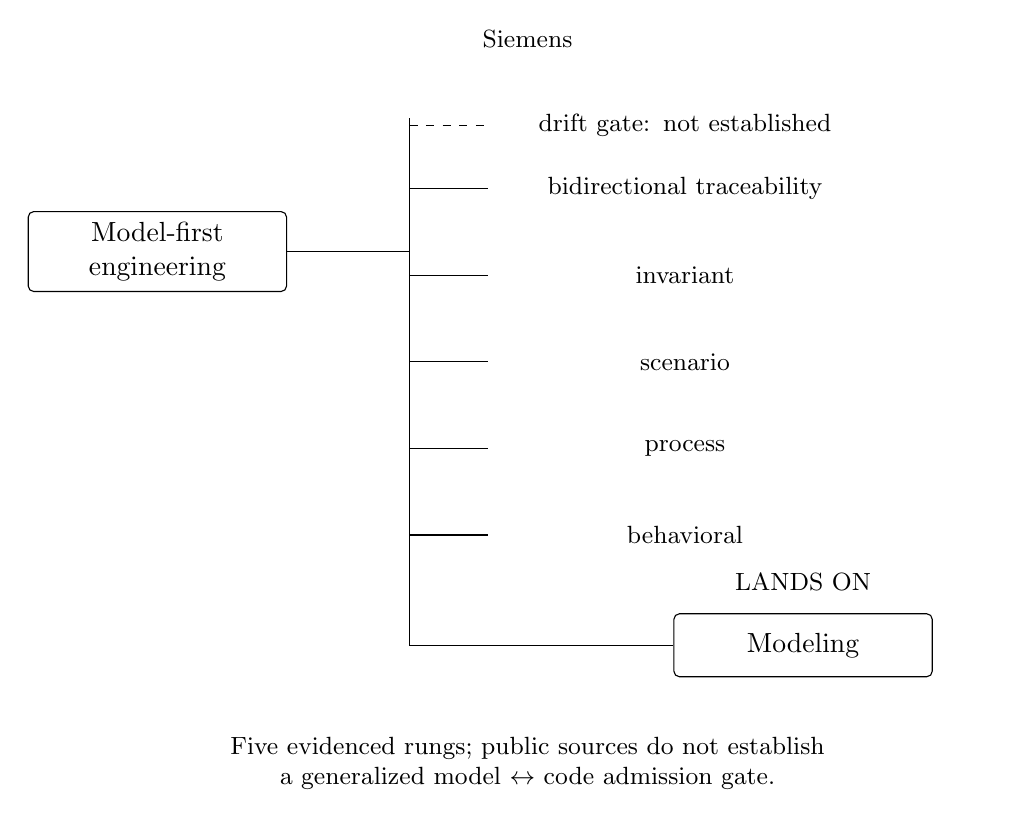
\begin{tikzpicture}[x=1cm,y=1cm,font=\magefigurefont\fontsize{10}{12}\selectfont,
box/.style={draw=black,fill=white,rounded corners=2pt,align=center,text width=3cm,minimum height=8mm,inner sep=4pt},
gate/.style={box,line width=1pt},note/.style={align=center,fill=white,inner sep=1pt,font=\magefigurefont\fontsize{9}{11}\selectfont},
edge/.style={-{Stealth[length=2mm]},line width=.6pt},optional/.style={edge,dashed},
every node/.style={text=black,execute at begin node={\hyphenpenalty=10000\exhyphenpenalty=10000}}]
\node[note,text width=12cm] (t5) at (0,2.7) {Siemens};
\node[box,text width=3cm] (entry) at (-4.7,0) {Model-first engineering};
\draw (-1.5,-3.6)--(-.5,-3.6);
\node[note,text width=4.5cm] (t8) at (2,-3.6) {behavioral};
\draw (-1.5,-2.5)--(-.5,-2.5);
\node[note,text width=4.5cm] (t10) at (2,-2.5) {process};
\draw (-1.5,-1.4)--(-.5,-1.4);
\node[note,text width=4.5cm] (t12) at (2,-1.4) {scenario};
\draw (-1.5,-0.2999999999999998)--(-.5,-0.2999999999999998);
\node[note,text width=4.5cm] (t14) at (2,-0.2999999999999998) {invariant};
\draw (-1.5,0.8000000000000003)--(-.5,0.8000000000000003);
\node[note,text width=4.5cm] (t16) at (2,0.8000000000000003) {bidirectional traceability};
\draw (-1.5,-4)--(-1.5,1.7);\draw[dashed] (-1.5,1.6)--(-.5,1.6);
\node[note,text width=4.5cm] (t18) at (2,1.6) {drift gate: not established};
\node[box,text width=3cm] (land) at (3.5,-5) {Modeling};\node[note,text width=12cm] at (0,-6.5) {Five evidenced rungs; public sources do not establish\\ a generalized model $\leftrightarrow$ code admission gate.};
\draw (entry.east)--(-1.5,0);\draw (-1.5,-4)--(-1.5,-5)--(land.west);\node[note] at (3.5,-4.2) {LANDS ON};
\end{tikzpicture}
